\documentclass[twocolumn, 10pt,a4j]{jsarticle}
\usepackage{here}
\usepackage{amsmath}
\usepackage[dvipdfmx]{graphicx}
\usepackage{url}
\title{\vspace{-2.5cm}8. 論理回路}
\author{1610581 堀田 大地}
\date{2018/5/17}
\begin{document}
\maketitle{}
\vspace{-10zh}
\section{目的}
% 目的
トランジスタ,IC等の半導体素子の発展と共に機械システムへのエレクトロニクスの導入が進み,
今やエレクトロニクスと関わりのない機械システムは考えられなくなった.特にコンピュータを始め,
その周辺機器,各種情報機器,NC工作機械, 家電製品等にはディジタル回路が多用されている.そこで,
実際に広く利用されているディジタル用ICを用いて,ディジタル回路,特に論理回路の基礎的事項について実験し,
ディジタルICの使い方,動作,設計法について理解する.
\section{方法}
% 方法
[1]を参考にしながら,各実験項目を進めた.
\section{実験項目}
% 実験項目
\subsection{ゲート回路}
% ゲート回路
6種類のゲート回路についての素子名称,動作表,回路の読み方,真理値表,論理式を表4.1に示した.
\subsection{2入力EX-ORゲート}
  % 2入力EX-ORゲート
  \subsubsection{EX-ORの機能}
    % EX-ORの機能
    回路図を図1,動作表,真理値表を表1,2,論理式を(1)に示した.
      % 図1
    \begin{figure}[H]
      \begin{center}
        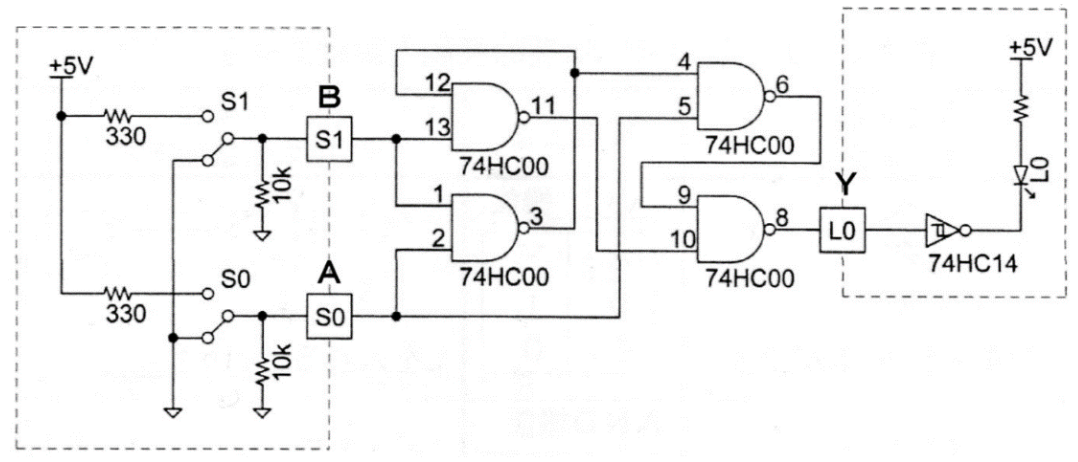
\includegraphics[width=7cm]{../img/ex_or/ex-or_kairo.png}
        \caption{NAND素子4個を用いたEX-OR機能の論理式}
      \end{center}
    \end{figure}
      % 表1 
    \begin{table}[]
      \centering
      \caption{EX-ORの回路の動作表.入力のHはスイッチON,出力のHはLEDの点灯を表す}
      \label{my-label}
      \footnotesize
      \begin{tabular}{l|ll|l}
            & 入力                      &    & 出力 \\ \hline
        接続端子 & \multicolumn{1}{l|}{$S_{0}$} & $S_{1}$ & $L_{0}$ \\ \hline
        端子名  & \multicolumn{1}{l|}{A}  & B  & Y  \\ \hline
            & \multicolumn{1}{l|}{L}  & L  & L  \\
        電圧   & \multicolumn{1}{l|}{L}  & H  & H  \\
            & \multicolumn{1}{l|}{H}  & L  & H  \\
            & \multicolumn{1}{l|}{H}  & H  & L 
      \end{tabular}
    \end{table}
      % 表2
    \begin{table}[]
      \centering
      \caption{EX-OR機能の真理値表}
      \label{my-label}
      \footnotesize
      \begin{tabular}{l|ll|l}
            & 入力                     &   & 出力 \\ \hline
        端子名 & \multicolumn{1}{l|}{A} & B & Y  \\ \hline
            & \multicolumn{1}{l|}{0} & 0 & 0  \\
        真理値 & \multicolumn{1}{l|}{0} & 1 & 1  \\
            & \multicolumn{1}{l|}{1} & 0 & 1  \\
            & \multicolumn{1}{l|}{1} & 1 & 0 
      \end{tabular}
    \end{table}
    
    \begin{center}
      $Y = A・\overline{B} + \overline{A} + B = A \oplus B$\quad(1)
    \end{center}
  \subsubsection{考察}
   % 考察
   実験では,$S_{0}$と$S_{1}$のうち1方がオンでのみ,LEDが点灯していたので,動作を確認できた.
   また,LEDの光り方により,EX-ORの回路の,出力A,BのうちどちらかがHでもう片方はLで出力YはHに,
   出力A,Bの両方がH,Lのとき出力YはLになるという機能は理解できた.
  \subsubsection{課題}
    % 課題
    実験で用いた回路を正論理/負論理のNAND素子を使って書き換えた回路を図2に示した.
    この課題では,図の回路の出力YがEX-OR機能であることを示した.
    C,$\overline{D}$,$\overline{E}$,Yの論理式を(2)-(5)に示した.
    % 図2
    \begin{figure}[H]
      \begin{center}
        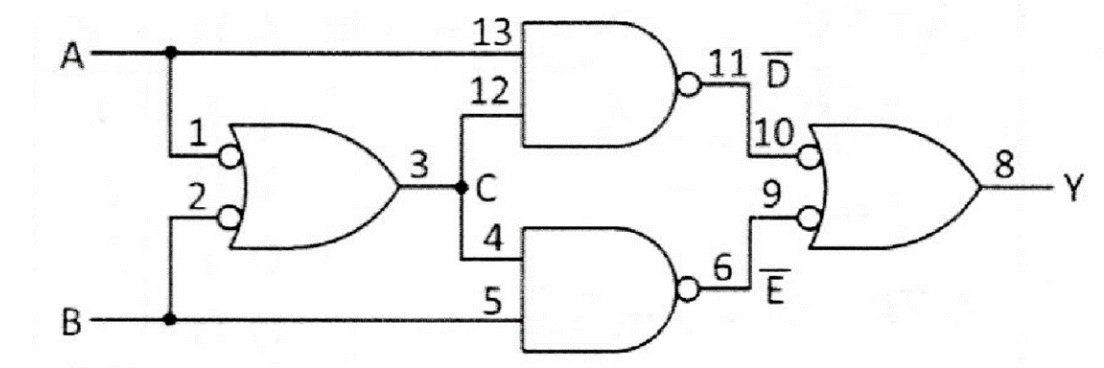
\includegraphics[width=7cm]{../img/ex_or/nand_ex_or_kairo.png}
        \caption{正論理/負論理のNAND素子を使って作ったEX-OR回路}
      \end{center}
    \end{figure}
      % 数式
    \begin{center}
        $C = \overline{A} + \overline{B}$\quad(2) \\
        $\overline{D} = A・C = A・(\overline{A} + \overline{B}) = A・\overline{B}$\quad(3) \\
        $\overline{E} = B・C = B・(\overline{A} + \overline{B}) = \overline{A}・B$\quad(4) \\
        $Y = \overline{D}+\overline{E}=A・\overline{B}+\overline{A}・B=A \oplus B$\quad(5) \\
    \end{center}
    よって, (5)より,図がEX-OR機能であることが示された.
\subsection{デコーダとエンコーダ}
% デコーダとエンコーダ
  \subsubsection{デコーダの機能}
  % デコーダの機能
  デコーダ回路は,2桁の2進数スイッチを使って入力し,10進数の0から3を表すLEDに"1(H)"を出力する.
  すなわち対応するLEDが点灯する回路である.
  回路図を図3,デコーダの動作表,真理値表を表3,4に示した.
   % 図3
  \begin{figure}[H]
    \begin{center}
      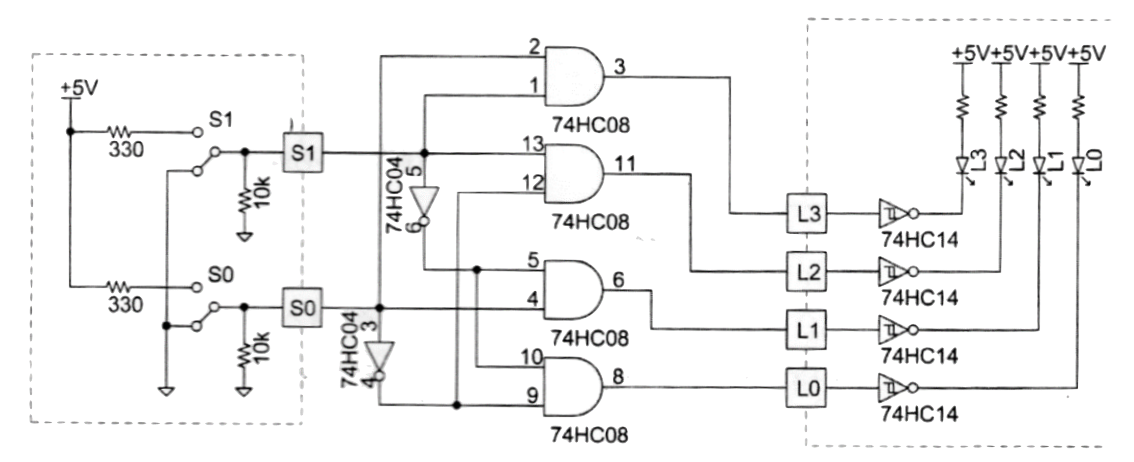
\includegraphics[width=7cm]{../img/decoda/input2_decoda.png}
      \caption{2入力4出力デコーダの回路図}
    \end{center}
  \end{figure}
  % 表3
  \begin{table}[H]
    \centering
    \caption{デコーダの動作表.入力のHはスイッチON,出力のHはLEDの点灯を表す.}
    \label{my-label}
    \footnotesize
      \begin{tabular}{l|ll|llll}
          & 入力 &    & 出力 &    &    &    \\ \hline
      端子名 & $S_{1}$ & $S_{0}$ & $L_{0}$ & $L_{1}$ & $L_{2}$ & $L_{3}$ \\ \hline
          & L  & L  & H  & L  & L  & L  \\
      電圧  & L  & H  & L  & H  & L  & L  \\
          & H  & L  & L  & L  & H  & L  \\
          & H  & H  & L  & L  & L  & H 
      \end{tabular}
  \end{table}
  % 表4
  \begin{table}[H]
    \centering
    \caption{デコーダの真理値表.
    入力の上位ビット,下位ビットを$S_{1}$,$S_{0}$,出力を$L_{x}$(x=0-3)が表す.}
    \label{my-label}
    \footnotesize
      \begin{tabular}{l|ll|llll}
          & 入力 &    & 出力 &    &    &    \\ \hline
      端子名 & S1 & S0 & L0 & L1 & L2 & L3 \\ \hline
          & 0  & 0  & 1  & 0  & 0  & 0  \\
      電圧  & 0  & 1  & 0  & 1  & 0  & 0  \\
          & 1  & 0  & 0  & 0  & 1  & 0  \\
          & 1  & 1  & 0  & 0  & 0  & 1 
      \end{tabular}
  \end{table}

  \subsubsection{考察}
  % 考察
  \begin{enumerate}
    \item 回路の動作についての考察 \\
      スイッチの位置と2進数表記の桁を合わせてH,Lを変えて行くと,
      LEDの位置を出力とみると,10進数となって動作していた.
    \item この回路の入力と出力の関係が「解読」であることの考察 \\
      $S_{0}$,$S_{1}$の2入力4通りの組み合わせによるすべての出力は異なり,
      $S_{0}$,$S_{1}$が2進数の1,2桁目を表しているとみると,出力はLEDが
      該当する番号が10進数に復元した数字ととらえると,出力結果を見るだけで,
      入力の信号がわかる.
      よって,入力と出力の関係が「解読」であると言える.
  \end{enumerate}
  \subsubsection{課題}
  % 課題
  エンコーダは10進数を2進数に変換する回路である.
  この課題では,10進数から0から3をそれぞれに対応する4つのスイッチ($S_{0}$,$S_{1}$,$S_{2}$,$S_{3}$)
  を使って入力し,2つのLED($L_{0}$,$L_{1}$)を使って2ビットの2進数を出力するエンコーダ回路を
  設計し作成した.
  まず,エンコーダの真理値表を表5に,論理式を(6),(7)に,回路図を図4に示した.
  % 表5
  \begin{table}[H]
  \centering
  \caption{エンコーダの真理値表}
  \label{my-label}
  \footnotesize
  \begin{tabular}{l|llll|ll}
      & 入力      &         &         &         & 出力      &         \\ \hline
  端子名 & $S_{0}$ & $S_{1}$ & $S_{2}$ & $S_{3}$ & $L_{1}$ & $L_{0}$ \\ \hline
      & 1       & 0       & 0       & 0       & 0    & 0    \\
  真理値 & 0       & 1       & 0       & 0       & 0    & 1    \\
      & 0       & 0       & 1       & 0       & 1    & 0    \\
      & 0       & 0       & 0       & 1       & 1    & 1   
  \end{tabular}
  \end{table}
  % 論理式
  \begin{center}
    $L_{0} = S_{1}+S_{3}$\quad(6) \\
    $L_{1} = S_{2}+S_{3}$\quad(7) \\
  \end{center}
  % 図4
  \begin{figure}[H]
    \begin{center}
      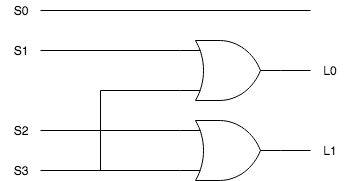
\includegraphics[width=7cm]{../img/half_adder/encoder.png}
      \caption{4入力2出力エンコーダの回路図}
    \end{center}
  \end{figure}
\subsection{加算回路}
% 加算回路
  \subsubsection{加算回路の機能}
    ハーフ・アダーは,2進数の足し算,つまり2つの入力AとBを加算し,その和S(Sum)と桁上げC(Carry)を出力する.
    ハーフ・アダーの真理値表,動作表を表6,7に,回路図を図5に,動作確認表を表7に,論理式を(8),(9)に示した.
    % 表6
    \begin{table}[]
      \centering
      \caption{ハーフ・アダーの真理値表}
      \label{my-label}
      \footnotesize
      \begin{tabular}{l|ll|ll|}
          & 入力 &   & 出力 &     \\ \cline{4-5} 
          &  &   & 和  & 桁上げ \\ \hline
      端子名 & A  & B & S  & C   \\ \hline
      真理値 & 0  & 0 & 0  & 0   \\
          & 0  & 1 & 1  & 0   \\
          & 1  & 0 & 1  & 0   \\
          & 1  & 1 & 0  & 1  
      \end{tabular}
    \end{table}
    % 図5
    \begin{figure}[H]
      \begin{center}
        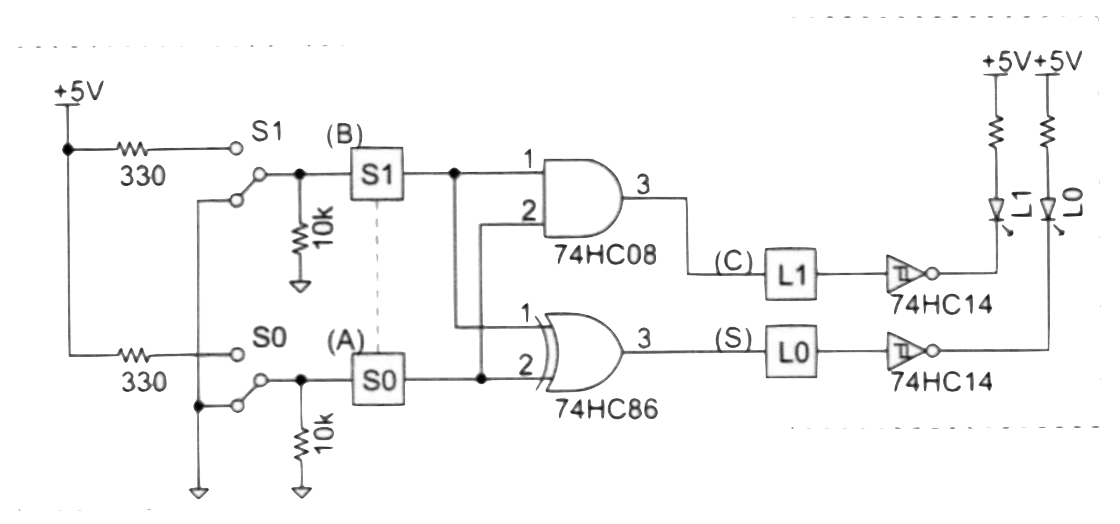
\includegraphics[width=7cm]{../img/half_adder/half_ader_kairo.png}
        \caption{ハーフ・アダーの回路図}
      \end{center}
    \end{figure}
    % 表7
    \begin{table}[H]
      \centering
      \caption{ハーフ・アダーの動作表}
      \label{my-label}
      \footnotesize
        \begin{tabular}{l|ll|ll|}
            & 入力      &         & 出力      &         \\ \cline{4-5} 
            &         &         & 和       & 桁上げ     \\ \hline
        接続端子 & $S_{0}$ & $S_{1}$ & $L_{0}$ & $L_{1}$ \\ \hline
        端子名  & A       & B       & S       & C       \\ \hline
        電圧   & L       & L       & L       & L       \\
            & L       & H       & H       & L       \\
            & H       & L       & H       & L       \\
            & H       & H       & L       & H      
        \end{tabular}
    \end{table}
    \begin{center}
      $S = A \oplus B$\quad(8) \\
      $C = A・B$\quad(9) \\  
    \end{center}
  \subsubsection{考察}
    % 考察
    和SがEX-OR,桁上げCがANDとなっており,$A=B=1$の時に,$S=0$,$C=1$となり,
    桁上げが行えた.
  \subsubsection{課題}
    コンピュータの内部では,複数桁同士の2進数の加算が行われている.
    この課題では,そのような計算を実現させるために,2桁の2進数の$A_{0}$,$A_{1}$と
    $B_{0}$,$B_{1}$との加算を行う回路を作成した.
    \begin{enumerate}
    \item 機能説明 \\
      % 機能説明
      2桁2進数の計算が行える.そのために,1桁目の加算を行い,次に2桁目の加算を実現させるために,1桁目はハーフ・アダー,
      2桁目は下位からの桁上げを考慮して入力できる全加算器を使った.
    \item フル・アダーの回路設計 \\
      フル・アダーの真理値表を表8に,論理式を(10),(11)に,回路図を図6に示した.
      % 表8
      \begin{table}[H]
        \centering
        \caption{フル・アダーの真理値表}
        \label{my-label}
        \footnotesize
        \begin{tabular}{l|lll|ll}
            & 入力 &   &          & 出力 &           \\ \cline{5-6} 
            &    &   &          & 和  & 桁上げ       \\ \hline
        端子名 & A  & B & $C_{in}$ & S  & $C_{out}$ \\ \hline
        電圧  & 0  & 0 & 0        & 0  & 0         \\
            & 0  & 1 & 0        & 1  & 0         \\
            & 1  & 0 & 0        & 1  & 0         \\
            & 1  & 1 & 0        & 0  & 1         \\
            & 0  & 0 & 1        & 1  & 0         \\
            & 0  & 1 & 1        & 0  & 1         \\
            & 1  & 0 & 1        & 0  & 1         \\
            & 1  & 1 & 1        & 1  & 1        
        \end{tabular}
      \end{table}
      % 論理式
      \begin{center}
        \begin{eqnarray*}
          S &=& \overline{A}・B・\overline{C_{in}} + A・\overline{B}・\overline{C_{in}}
           + \overline{A}・\overline{B}・C_{in} + A・B・C_{in} \\
          &=& (A \oplus B) \oplus C_{in} \quad(10) \\
        \end{eqnarray*}
        \begin{eqnarray*}
          C_{out} &=& A・B・\overline{C_{in}} + \overline{A}・B・C_{in}
           + A・\overline{B}・C_{in} + A・B・C_{in} \\
          &=& A・B + (A \oplus B)・C_{in} \quad(11) \\
        \end{eqnarray*}
      \end{center}
      % 図6
      \begin{figure}[H]
        \begin{center}
          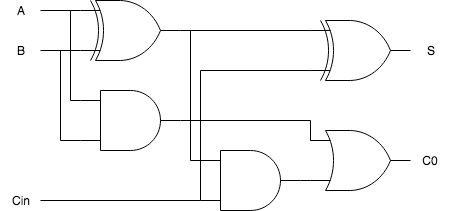
\includegraphics[width=7cm]{../img/half_adder/fullAdder.png}
          \caption{フル・アダーの回路図}
        \end{center}
      \end{figure}
    \item 2桁の2進数の加算回路の設計 \\
      真理値表を表9に,論理式を(12)-(14)に,回路図を図7に示した.
      % 表9
      \begin{table}[H]
      \centering
      \caption{2桁の2進数の加算回路の真理値表}
      \label{my-label}
        \footnotesize
        \begin{tabular}{l|llll|lll}
            & 入力      &         &         &         & 出力      &         &         \\ \cline{6-8} 
            &         &         &         &         & 3桁目     & 2桁目     & 1桁目     \\ \hline
        端子名 & $A_{1}$ & $A_{0}$ & $B_{1}$ & $B_{0}$ & $C_{2}$ & $S_{1}$ & $S_{0}$ \\ \hline
        真理値 & 0       & 0       & 0       & 0       & 0       & 0       & 0       \\
            & 0       & 1       & 0       & 0       & 0       & 0       & 1       \\
            & 1       & 0       & 0       & 0       & 0       & 1       & 0       \\
            & 1       & 1       & 0       & 0       & 0       & 1       & 1       \\
            & 0       & 0       & 0       & 1       & 0       & 0       & 1       \\
            & 0       & 1       & 0       & 1       & 0       & 1       & 0       \\
            & 1       & 0       & 0       & 1       & 0       & 1       & 1       \\
            & 1       & 1       & 0       & 1       & 1       & 0       & 0       \\
            & 0       & 0       & 1       & 0       & 0       & 1       & 0       \\
            & 0       & 1       & 1       & 0       & 0       & 1       & 1       \\
            & 1       & 0       & 1       & 0       & 1       & 0       & 0       \\
            & 1       & 1       & 1       & 0       & 1       & 0       & 1       \\
            & 0       & 0       & 1       & 1       & 0       & 1       & 1       \\
            & 0       & 1       & 1       & 1       & 1       & 0       & 0       \\
            & 1       & 0       & 1       & 1       & 1       & 0       & 1       \\
            & 1       & 1       & 1       & 1       & 1       & 1       & 0      
        \end{tabular}
      \end{table}
      $S_{0} = A_{0} \oplus B_{0} $\quad(12) \\
      $S_{1} = A_{0}・(A_{1} \oplus B_{1} \oplus B_{0}) + \overline{A_{0}}・(A_{1} \oplus B_{1})$ \quad(13) \\
      $C_{2} = A_{0}・B_{0}(A_{1} \oplus B_{1}) + A_{1}・B_{1}$ \quad(14) \\
      % 図7
      \begin{figure}[H]
        \begin{center}
          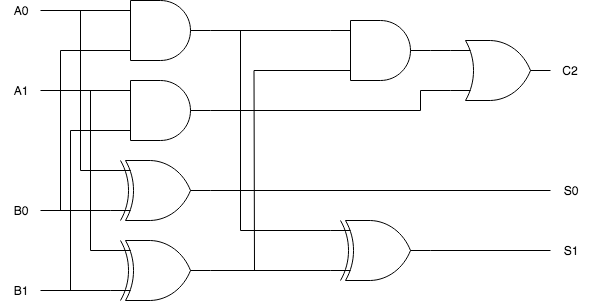
\includegraphics[width=7cm]{../img/half_adder/ronri.png}
          \caption{2桁の2進数の加算回路図}
        \end{center}
      \end{figure}
    \end{enumerate}
\subsection{順序回路}
  順序回路とは,組み合わせ回路の時刻$t+1$の時の出力$Y_{t+1}$が,時刻$t$のときの出力
  $Y_{t}$を含む入力条件によって決まる$Y_{t+1} = f(Y_{t},A,B,C...)$で表すことのできる回路である.
  \subsubsection{Dラッチ回路}
  % Dラッチ回路
    \begin{enumerate}
      \item 基本動作 \\
      % 基本動作
      Dラッチ回路は,RSラッチ(Reset入力とSet入力を持つラッチ)の前段にデータ記憶用の
      ゲートを追加し,入力したDataを止めるため,つまりラッチするための信号である
      ストローブ入力を備えている.つまり,Dラッチは,ストローブ入力によりデータをRSラッチ
      にいつ記憶させるかを制御している.回路図を図8に,動作表を表10に,タイムチャートを図9に示した.
      % 図8
      \begin{figure}[H]
        \begin{center}
          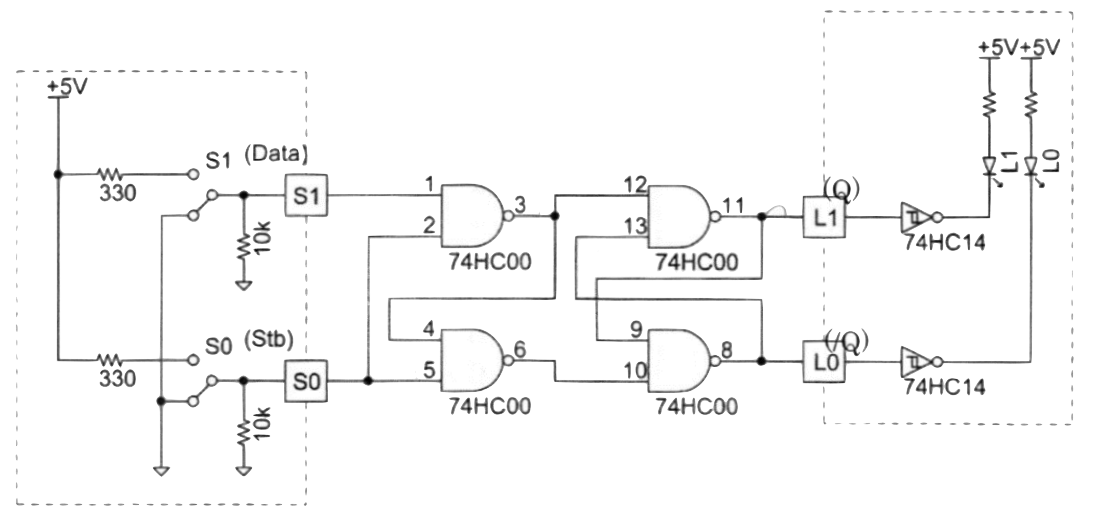
\includegraphics[width=7cm]{../img/junjokairo/d_ratch.png}
          \caption{Dラッチの回路図}
        \end{center}
      \end{figure}
      % 表10
      \begin{table}[H]
        \centering
        \caption{Dラッチの動作表}
        \label{my-label}
        \footnotesize
          \begin{tabular}{l|ll|ll}
              & 入力      &                                 & 出力                           &                                      \\ \hline
          接続端子 & $S_{1}$ & $S_{0}$                         & $L_{1}$ & $L_{0}$                              \\ \hline
          端子名  & Data    & $\overline{Stb}$              & Q       & $\overline{Q}$        \\ \hline
          電圧   & L       & L                               & $Q_{0}$ & $\overline{Q_{0}}$ \\
              & H       & L                               & $Q_{0}$ & $\overline{Q_{0}}$ \\
              & L       & H                               & L       & H                                    \\
              & H       & H                               & H       & L                                   
          \end{tabular}
      \end{table}
      % 図9
      \begin{figure}[H]
        \begin{center}
          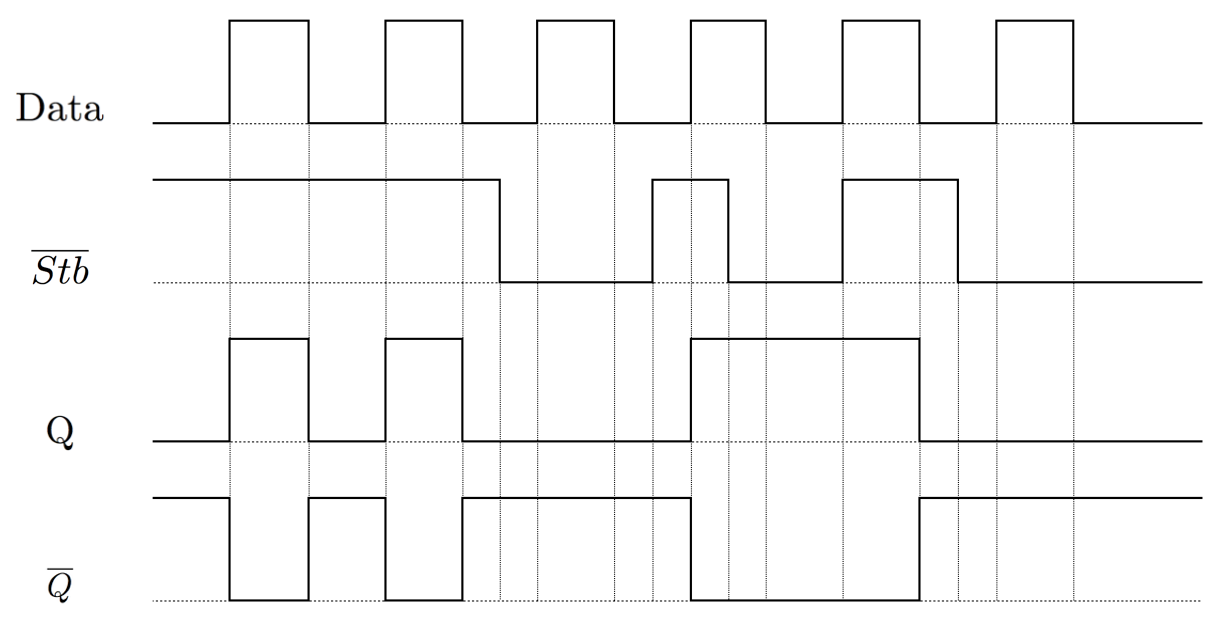
\includegraphics[width=7cm]{../img/junjokairo/d_ratchTimeChart.png}
          \caption{Dラッチのタイムチャート}
        \end{center}
      \end{figure}
      \item 考察
        % 考察
        \begin{enumerate}
          \item ストローブ信号がHのとき,Data信号の出力をQは受けとって出力していた.
          \item ストローブ信号がLのとき,Data信号の出力に関わらず,前の状態を維持していた. 
          \item Data信号が動いているときに,ストローブ信号をHからLにしたとき,
          Data信号の動きに関わらず出力Qの状態は変わらなかった.
          \item 以上の(a)-(b)より,ストローブ信号の機能は,Data信号を出力に伝える機能であった.
          ラッチ機能は,ストローブ機能がLのときに,Data信号を止めて,もしData信号が変わっても
          受け取らないようにするための機能であった.
        \end{enumerate}
    \end{enumerate}
  \subsubsection{フリップフロップ回路}
  % フリップフロップ回路
    \begin{enumerate}
      \item J-Kフリップフロップ回路(74HC112)
        \begin{enumerate}
          \item 基本動作 \\
            J-Kフリップフロップ回路とは,入力端子J,Kの組み合わせにより,
            出力端子Q,その反転出力である$\overline{Q}$にクロックを同期して新しい状態を出力できる回路である.
            基本動作は,リセット,セット,維持,反転の4パターンである.回路図を図10に,動作表を表11に示した.
            % 図10
            \begin{figure}[H]
              \begin{center}
                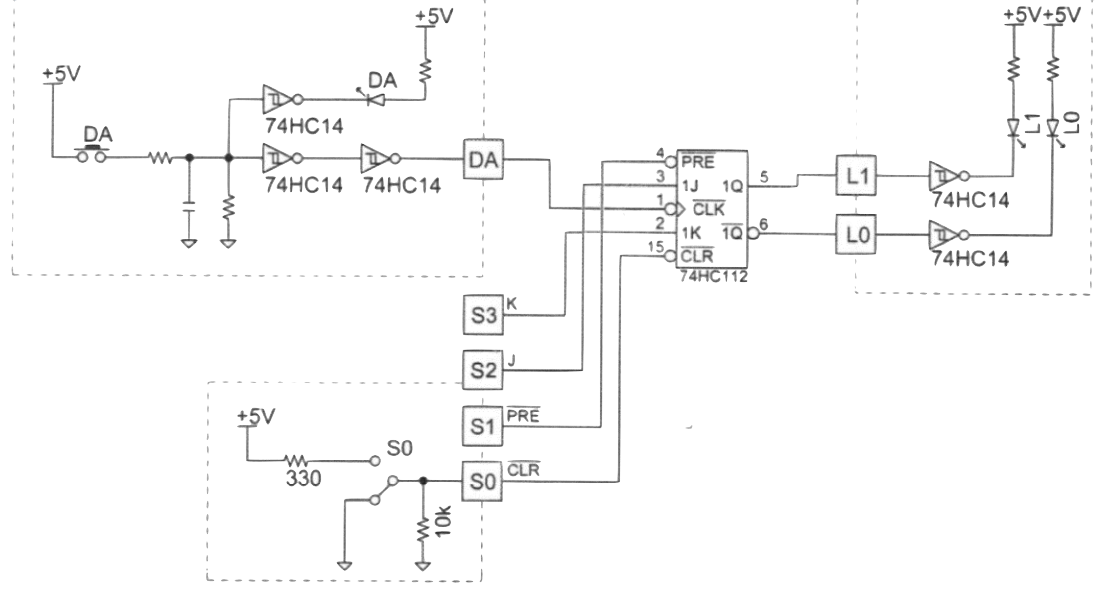
\includegraphics[width=7cm]{../img/junjokairo/jk_flip_flop.png}
                \caption{J-Kフリップフロップ回路の回路図}
              \end{center}
            \end{figure}
            % 表11
            \begin{table}[H]
              \centering
              \caption{J-Kフリップフロップ回路の回路図の入出力端子と動作表}
              \label{my-label}
                \footnotesize
                \begin{tabular}{lllll|ll|ll}
                入力      &         &         &         &     & 出力      &         & 機能        \\ \cline{1-7}
                $S_{0}$ & $S_{1}$ & $S_{2}$ & $S_{3}$ & DA  & $L_{1}$ & $L_{0}$ &               \\ \cline{1-7}
                $\overline{CLR}$  & $\overline{PR}$   & J   & K       & $\overline{CLK}$ & Q & $\overline{Q}$ &  \\ \hline
                L       & H       & x       & x       & x   & L       & H       & クリア  \\
                H       & L       & x       & x       & x   & H       & L       & プリセット  \\
                L       & L       & x       & x       & x   & H*      & H*      & 不定.  \\
                H       & H       & L       & L       & ↓   & $Q_{0}$ & $\overline{Q_{0}}$ & $t_{0}$の状態を保持 \\
                H       & H       & L       & H       & ↓   & L       & H       & ラッチ J→Q \\
                H       & H       & H       & L       & ↓   & H       & L       & K→Q \\
                H       & H       & H       & H       & ↓   & $\overline{Q_{0}}$ & $Q_{0}$ & トグル \\
                H       & H       & x       & x       & H   & $Q_{0}$ & $\overline{Q_{0}}$ & 
                \end{tabular}
            \end{table}
          \item 実験 \\
            図11に,タイムチャートに従って入力端子を操作したときの出力Q,$\overline{Q}$を示した.
            % 図11
            \begin{figure}[H]
              \begin{center}
                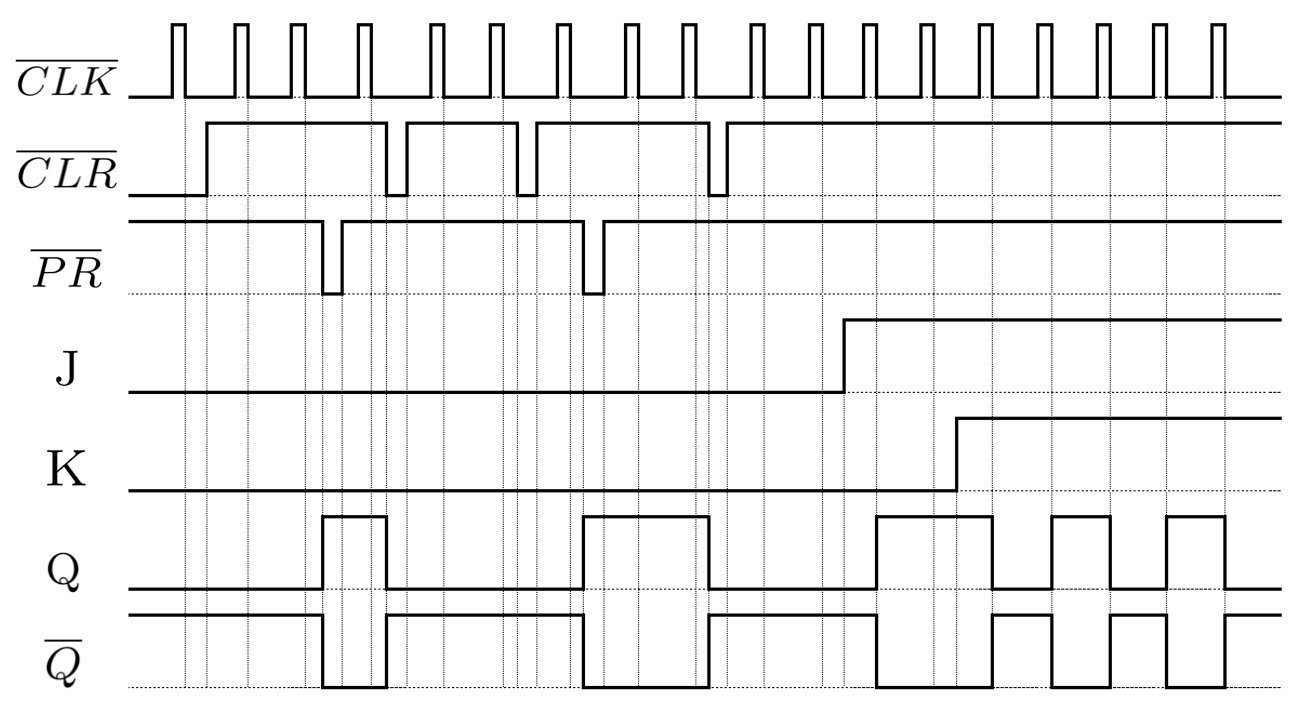
\includegraphics[width=7cm]{../img/junjokairo/jk_flip_flop_time_chart.png}
                \caption{J-Kフリップフロップ回路のタイムチャート}
              \end{center}
            \end{figure}
          \item 考察 \\
            % 考察
            出力Q,$\overline{Q}$は,$\overline{CLR}$がHで$\overline{PR}$がLになったとき,H,Lになった.
            逆に,$\overline{PR}$がHの状態で$\overline{CLR}$がLになったとき,L,Hになった.
            つまりこの2点から,$\overline{CLR}$はLになると,QをLに,$\overline{Q}$をHに変え,
            $\overline{PR}$はLになると,QをHに,$\overline{Q}$をLに変えていると考えられた.
            $\overline{CLR}$,$\overline{PR}$をHのまま,JをH,KをLの状態にして,
            $\overline{CLK}$をLにすると,QがH,$\overline{Q}$がLになったことより,
            タイムチャート前半の$\overline{PR}$の機能を呼び出せられると考えられた.
            また,その状態のままJをL,KをHにして,$\overline{CLK}$をLにすると,
            $\overline{CLR}$の機能を呼び出せられると考えられた.
            J,Kを両方Hにすると,$\overline{CLK}$をLにする度,前の状態が復元されると考えられた.
        \end{enumerate}
      \item Dフリップフロップ回路(74HC74)を用いた$1/2$分周器
        \begin{enumerate}
          \item 実験
          % 実験
          Dフリップフロップの動作表を表12に,Dフリップフロップ回路を用いた$1/2$分周器の回路図を図12に,
          動作表を表13に,タイムチャートを図13に示した
          % 表12
          \begin{table}[H]
            \centering
            \caption{Dフリップフロップ回路(74HC74)}
            \label{my-label}
            \footnotesize
            \begin{tabular}{llll|ll|l}
            入力  &    &   &     & 出力 &    & 機能         \\ \hline
            $\overline{CLR}$ & $\overline{PR}$ & D & CLK & Q  & $\overline{Q}$ &            \\ \hline
            L   & H  & x & x   & L  & H  & クリア   \\
            H   & L  & x & x   & H  & L  & プリセット \\
            L   & L  & x & x   & H* & H* & 不定         \\
            H   & H  & L & ↑   & L  & H  & D→Q        \\
            H   & H  & H & ↑   & H  & L  & D→Q        \\
            H   & H  & x & L   & $Q_{0}$ & $\overline{Q_{0}}$ & $t_{0}$の状態を保持  
            \end{tabular}
          \end{table}
          % 図12
          \begin{figure}[H]
              \begin{center}
                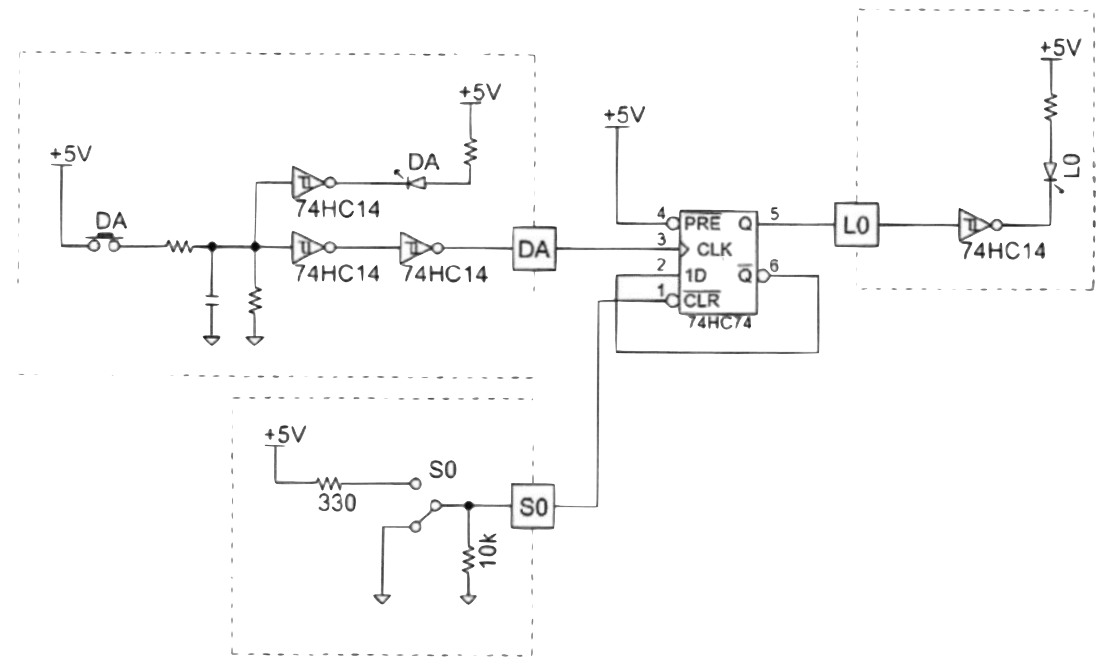
\includegraphics[width=7cm]{../img/junjokairo/d_ff.png}
                \caption{Dフリップフロップ回路を用いた$1/2$分周器の回路図}
              \end{center}
          \end{figure}
          % 表13
          \begin{table}[]
            \centering
            \caption{Dフリップフロップ回路を用いた$1/2$分周器の動作表}
            \label{my-label}
            \footnotesize
            \begin{tabular}{l|ll|l}
                  & 入力  &     & 出力 \\ \hline
              接続端子 & $S_{0}$  & DA  & $L_{0}$ \\ \hline
              端子名  & $\overline{CLR}$ & CLK & Q  \\ \hline
              クリア  & L   & x   &    \\ \hline
              分周機能 & H   & 0L  & L  \\
                  & H   & 1↑  & H  \\
                  & H   & 2↑  & L  \\
                  & H   & 3↑  & H  \\
                  & H   & 4↑  & L  \\
                  & H   & 5↑  & H  \\
                  & H   & 6↑  & L 
            \end{tabular}
          \end{table}
          % 図13
          \begin{figure}[H]
              \begin{center}
                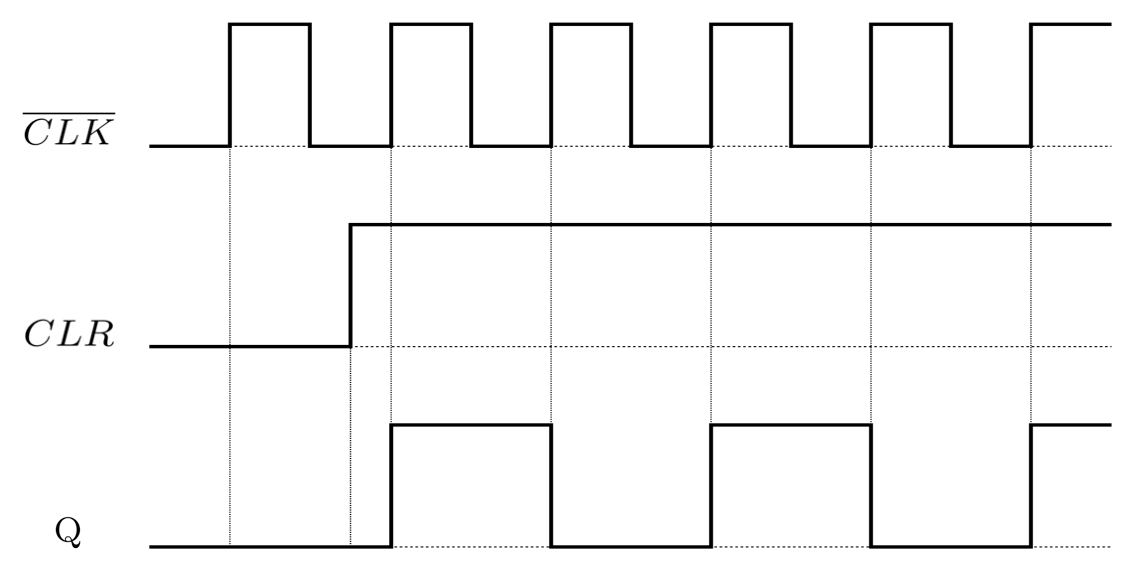
\includegraphics[width=7cm]{../img/junjokairo/d-ff_time_chart.png}
                \caption{Dフリップフロップを用いた$1/2$分周器のタイムチャート}
              \end{center}
          \end{figure}
          \item 考察
            \begin{enumerate}
              \item $\overline{CLR}$がHのときのみ,CLKがLからHになったときに,出力Qが反転した.
              \item $\overline{CLR}$の2周期分がQの1周期に相当していたので,出力Qは$\overline{CLR}$の倍の周期であった.
              \item 周波数は,周期の逆数なので,出力Qは$\overline{CLR}$の1/2倍の周期であった.
              \item 以上の3点より,分周器の分周機能とは,周波数を整数分の1にする機能であると考えられた.
            \end{enumerate}
        \end{enumerate}
    \end{enumerate}
\subsection{カウンタ回路}
% 非同期16進カウンタ回路
  \subsubsection{非同期16進カウンタ回路}
  非同期16進カウンタ回路とは,J-Kフリップフロップ回路を4つ用いた回路である.
  回路図,タイムチャートを図14,15に,動作表を表14に示した.
  % 図14
  \begin{figure}[H]
    \begin{center}
      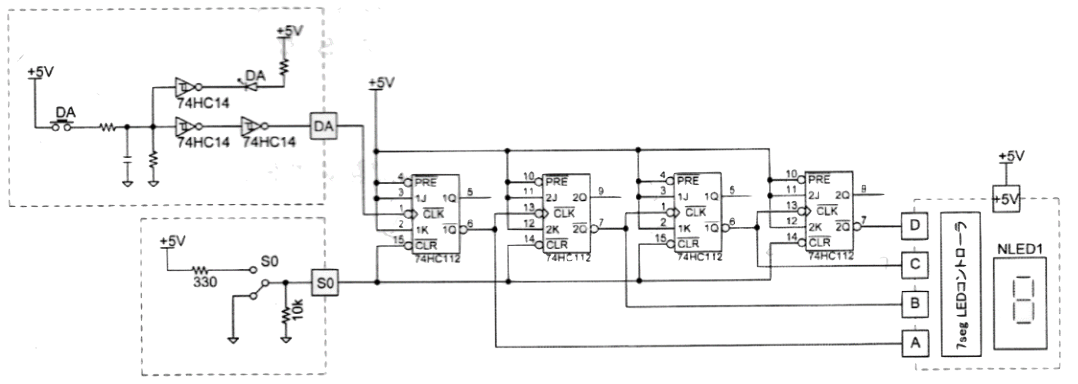
\includegraphics[width=7cm]{../img/junjokairo/hidouki_16sin_kairozu.png}
      \caption{非同期16進カウンタの回路図}
    \end{center}
  \end{figure}
  % 表14
  \begin{table}[H]
    \centering
    \caption{非同期16進カウンタの動作表}
    \label{my-label}
      \footnotesize
      \begin{tabular}{lllllll}
        $\overline{CLR}$ & $\overline{CLK}$ & D  & C  & B  & A  & NLED1 \\
        $S_{0}$  & DA  & $L_{3}$ & $L_{2}$ & $L_{1}$ & $L_{0}$ & \\ \hline
        L   & X   & H  & H  & H  & H  & F     \\
        H   & L   & H  & H  & H  & H  & F     \\
        H   & 1↓  & L  & L  & L  & L  & 0     \\
        H   & 2↓  & L  & L  & L  & H  & 1     \\
        H   & 3↓  & L  & L  & H  & L  & 2     \\
        H   & 4↓  & L  & L  & H  & H  & 3     \\
        H   & 5↓  & L  & H  & L  & L  & 4     \\
        H   & 6↓  & L  & H  & L  & H  & 5     \\
        H   & 7↓  & L  & H  & H  & L  & 6     \\
        H   & 8↓  & L  & H  & H  & H  & 7     \\
        H   & 9↓  & H  & L  & L  & L  & 8     \\
        H   & 10↓ & H  & L  & L  & H  & 9     \\
        H   & 11↓ & H  & L  & H  & L  & 10    \\
        H   & 12↓ & H  & L  & H  & H  & b     \\
        H   & 13↓ & H  & H  & L  & L  & c     \\
        H   & 14↓ & H  & H  & L  & H  & d     \\
        H   & 15↓ & H  & H  & H  & L  & E     \\
        H   & 16↓ & H  & H  & H  & H  & F     \\
        H   & 17↓ & L  & L  & L  & L  & 0    
      \end{tabular}
    \end{table}
  % 図15
  \begin{figure}[H]
    \begin{center}
      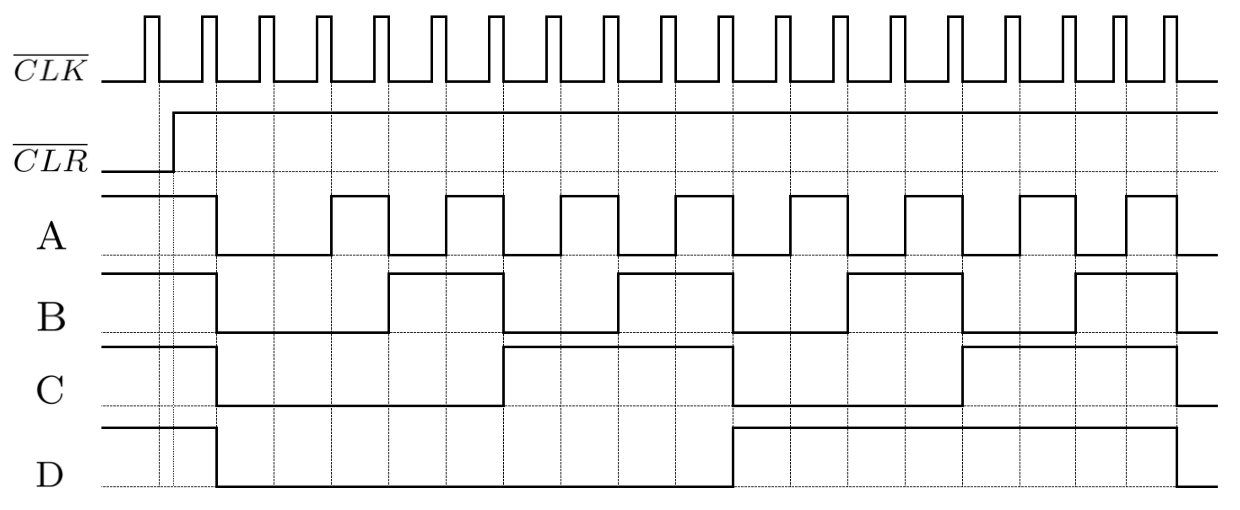
\includegraphics[width=7cm]{../img/junjokairo/hidouki_16shin_dousahyou.png}
      \caption{非同期16進カウンタのタイムチャート}
    \end{center}
  \end{figure}
  \begin{enumerate}
    \item 機能説明 \\
    % 入力の操作と出力の動作の関係について説明することである
    2つの入力$\overline{CLK}$,$\overline{CLR}$と4つの出力A,B,C,Dがある.
    1段目の出力$\overline{1Q}$は出力AとしてNLED1に接続され,同時に2段目の入力
    $\overline{CLK}$に接続されている.2段目の出力$\overline{2Q}$は出力Bとして
    NLED1に接続され,同時に3段目の入力$\overline{CLK}$に接続されている.
    3段目の出力$\overline{1Q}$は出力CとしてNLED1に接続され,同時に4段目の
    入力$\overline{CLK}$に接続されている.最後に,4段目の出力$\overline{2Q}$
    は出力DとしてNLED1に接続されている.もう1つの入力$\overline{CLR}$は,
    1段目から4段目のJ-Kフリップフロップの$\overline{CLR}$に同時に接続されている.
    さらに,4つの出力A,B,C,DをそれぞれLEDの$L_{0}$,$L_{1}$,$L_{2}$,$L_{3}$にも
    接続する.

    \item 考察 \\
      \begin{enumerate}
        \item 
          $S_{0}$をLにすると,$\overline{CLK}$に関わらず4つの出力A,B,C,DはHに,NLED1はFになった.
          Fはリセットの機能である.
        \item 
          $\overline{CLR}$をHにした後,入力$\overline{CLK}$に立下り信号を入力すると,
          4つの出力は全てLになり,NLED1はFになった
        \item 
          さらに,$\overline{CLK}$をに立下り信号を入力し続けると,
          最初の1回はどの出力もLのままだったが,2回目以降は,
          出力Aは,$\overline{CLK}$がLになるタイミング毎回,
          出力Bは,2回に1回,
          出力Cは,4回に1回,
          出力Dは,8回に1回,
          NLED1は,16進数表記で1ずつ加算されているように変化していた.
        \item 
          4つの出力を,DCBAの順番にしたとき,この出力をHを1,Lを0とし,
          D,C,B,Aを4,3,2,1桁目を表しているとみると,
          2進数で数字を表現していると考えられた.
        \item 
          入力$\overline{CLK}$と出力Aの周期の間には,
          $1 : 2 = \overline{CLK} : A$の関係があると考えられた.
          また,出力AとB,BとC,CとDの間には,$1 : 2 = A : B $,
          $1 : 2 = B : C $,$1 : 2 = C : D $の関係があると考えられた.
          さらに,入力$\overline{CLK}$信号の周期を基準とすると,各周期の大きさの比は$1 : 2 : 4 : 8 :16= \overline{CLK} : A:B:C:D$
          であった.
        \item 
          入力$\overline{CLK}$と出力Aの周波数の間には,周波数は周期の逆数なことを考慮すると,
          $1 : 1/2 = \overline{CLK} : A$の関係があると考えられた.
          また,出力AとB,BとC,CとDの間には,$1 : 1/2 = A : B $,
          $1 : 1/2 = B : C $,$1 : 1/2 = C : D $の関係があると考えられた.
          さらに,入力$\overline{CLK}$信号の周期を基準とすると,各周波数の大きさの比は$1 : 1/2 : 1/4 : 1/8 : 1/16= \overline{CLK} : A:B:C:D$
          であった.
          

      \end{enumerate}
    
  \end{enumerate}
\section{感想}
% 感想
理論的にはわかっていた論理回路を実際にブレッドボード上で実装してみることで,
各ゲートの組み合わせで論理回路を実装できることに感動した.
また,順序回路は現在の入力値だけでなく,過去に入力された値によって出力値を決定する論理回路であり,
その回路を実装してみて,結果を見ていくと本当になっていることがわかったのはとても感動した.

\begin{thebibliography}{3}
  \bibitem{}知能機械工学基礎実験テキスト P.52-P.80
  \bibitem{}CT-311S 実習セット(デジタル編)学習の手引き,サンハヤト株式会社
  \bibitem{}最新74シリーズIC規格票,CQ出版社
  \bibitem{}猪飼國夫,本多中二共著,定本 ディジタルシステムの設計,CQ出版社
\end{thebibliography}
\end{document}